% Template for a Thesis
%
% 5-methodology.tex
%
% Methodology

\chapter{Methodology}\label{sec:methodology}

Theoretical idea: what I want to do, how, algorithmic/mathematical

This chapter explains the technical content of this thesis in broad strokes, the methodology used and the general idea of the methods employed. For a more in-depth analysis, refer to the next chapter.

This thesis, first of all, aims to replicate the results of BPE and BPE dropout.

\section{Replication of BPE results}

Using Sennrich et al.'s~\cite{sennrich2015neural} \href{code on Github}{https://github.com/rsennrich/subword-nmt/}, the first goal was to check the gold standard's alignment scores. For that, these steps were undertaken:

\begin{enumerate}
	\item Write learn BPE from corpus algorithm
	\item Write apply BPE to corpus algorithm
	\item Write extract alignment script
	\item Write calculate alignment scores script
\end{enumerate}

The actual code for each step can be found in the next section, Development.

The corpus is a 10k sentence English-German corpus, containing an index number for each sentence. As an excerpt of the corpora:

\begin{quote}
	English\\
	21	The Committee on Transport and Tourism has adopted four amendments for the second reading .\\
	22	They will certainly enhance the feeling of the right of movement by EU citizens and they will also certainly benefit disabled drivers .\\
	23	The initial Commission proposal was adopted unamended by Parliament on first reading .\\\\
	German\\
	21	Der Transportausschuß hat für die zweite Lesung vier Änderungsanträge beschlossen .\\
	22	Sie werden bei den EU-Bürgern gewiß das Gefühl für das Recht auf Freizügigkeit stärken , und sie werden gewiß auch behinderten Fahrern Vorteile bringen .\\
	23	Der ursprüngliche Vorschlag der Kommission wurde vom Parlament in erster Lesung ohne Änderungen verabschiedet .
\end{quote}

\subsection{Learn BPE algorithm}

Sennrich's repository's code has some additional parameters that weren't relevant for a minimal implementation of the BPE algorithm, so the script was adapted. These are the steps for a minimal learn BPE algorithm:

\begin{enumerate}
	\item Read corpus into tokens, parse index.
	\item Count pair frequencies.
	\item Start loop from 1 until desired vocabulary size. In our case, 10k merges.
	\begin{enumerate}
		\item Get most frequent pair.
		\item Append most frequent pair to vocabulary.
		\item Merge pair in corpus.
		\item Count pair frequencies in corpus.
	\end{enumerate}
	\item Write vocabulary to a file.
\end{enumerate}

This step of the pipeline only has to be done once for each corpus, afterwards the vocabulary can be used in different ways. But this minimal algorithm, since it has to count all the pairs in the whole corpus in each iteration, takes a long time. An optimization came after this.

With the given corpus, these are the 10 most frequent merges in the English language:

\begin{enumerate}
	\item \_t h
	\item \_th e
	\item o n
	\item r e
	\item t i
	\item e n
	\item e r
	\item i n
	\item i s
	\item n d
\end{enumerate}

And the 10 most frequent merges in German:

\begin{enumerate}
	\item e n
	\item e r
	\item c h
	\item i e
	\item e i
	\item n d
	\item n g
	\item \_d ie
	\item s t
	\item i ch
\end{enumerate}

\subsection{Apply BPE algorithm}

Once the vocabulary has been learnt, it can be applied to a corpus. In this case, we use the same corpus for training and for applying. To generate different output files, different num\_merges are declared. For example, for 500 merges, only the first 500 merges of the vocabulary are considered, and there aren't many recognizable BPE units in the corpus. For bigger merge values, more and more subword units get merged. In this thesis, the following merges have been considered: [100, 200, 500, 1000, 2000, 4000, 6000, 8000]. These are the steps for this part:

\begin{enumerate}
	\item Load data, corpus and BPE vocabulary.
	\item Start loop for all numbers of merges.
	\begin{enumerate}
		\item Start loop from 1 until desired amount of merges.
		\begin{enumerate}
			\item Merge corpus for current most frequent pair.
		\end{enumerate}
		\item Write to output.bpe file.
	\end{enumerate}
\end{enumerate}

For example, this is what the excerpt from the corpora above look like after 100 merges:

\begin{quote}
	English\\
	\_the \_Comm it t e e \_on \_T ran s p ort \_and \_T ouris m \_has \_a d o p t ed \_f our \_a m end ment s \_for \_the \_sec ond \_re a d ing \_.\\
	\_the y \_w ill \_cer t a in ly \_en h an ce \_the \_f e e ling \_of \_the \_ri g h t \_of \_m o ve ment \_b y \_E U \_citi z en s \_and \_the y \_w ill \_al s o \_cer t a in ly \_ben e f it \_d is a bled \_d ri ver s \_.\\
	\_the \_in iti al \_Commission \_pro p o s al \_w as \_a d o p t ed \_u n a m end ed \_b y \_P ar li a ment \_on \_f ir st \_re a d ing \_.\\\\
	German\\
	\_der \_T rans p or t a ussch u ß \_h at \_für \_die \_z w eite \_L es ung \_v ier \_Ä nder ung s ant r ä ge \_besch l o ss en \_.\\
	\_s ie \_wer den \_bei \_den \_E U - B ür ger n \_ge w i ß \_das \_G e f ü h l \_für \_das \_Re ch t \_auf \_F r ei z ü g i g k eit \_st ä r k en \_, \_und \_s ie \_wer den \_ge w i ß \_au ch \_beh inder ten \_F a hr er n \_V or tei l e \_b r ingen \_.\\
	\_der \_ur s p r ü ng lich e \_V or sch la g \_der \_Ko mm iss ion \_w ur de \_v o m \_P ar la ment \_in \_er ster \_L es ung \_o h n e \_Ä nder ungen \_vera b sch ie det \_.
\end{quote}

Only the 100 most common units in the language have been merged, so in English we can see the merge of \emph{\_the}, \emph{\_and}, \emph{ment}, and other very common words and affix/suffixes. As for German, we can see very common words being merged such as \emph{\_die}, \emph{\_das}, \emph{\_bei} and so on. When we do 4000 merges:

\begin{quote}
	English\\
	\_the \_Committee \_on \_Transport \_and \_Tourism \_has \_adopted \_four \_amendments \_for \_the \_second \_reading \_.\\
	\_they \_will \_certainly \_enhance \_the \_feeling \_of \_the \_right \_of \_movement \_by \_EU \_citizens \_and \_they \_will \_also \_certainly \_benefit \_dis abled \_drivers \_.\\
	\_the \_initial \_Commission \_proposal \_was \_adopted \_un amended \_by \_Parliament \_on \_first \_reading \_.\\\\
	German\\
	\_der \_T ransp ortausschuß \_hat \_für \_die \_zweite \_Lesung \_vier \_Änderungsanträge \_beschlossen \_.\\
	\_sie \_werden \_bei \_den \_EU-B ür gern \_gew iß \_das \_Ge fü hl \_für \_das \_Recht \_auf \_Freizügigkeit \_stärken \_, \_und \_sie \_werden \_gew iß \_auch \_behinderten \_Fahrern \_Vorteile \_bringen \_.\\
	\_der \_ursprüngliche \_Vorschlag \_der \_Kommission \_wurde \_vom \_Parlament \_in \_erster \_Lesung \_ohne \_Änderungen \_verabschiedet \_.
\end{quote}

Most words are merged, except \emph{\_dis abled} in English, and \emph{\_T ransp ortausschuß} in German for instance.

\subsection{Extract alignments}\label{subsec:extractalign}

Write extract alignment script to align files from 2 different languages using fastalign/eflomal

To evaluate if the BPE units are good, bilingual corpora are aligned, and then compared against a gold standard. On the first step, alignment, two algorithms have been used, fastalign and eflomal. The software installation guides can be found in the development section.

These algorithms take English text and German as input and create an alignment file as output. For the example above:

\begin{quote}
	English sentence: The Committee on Transport and Tourism has adopted four amendments for the second reading .\\
	German sentence: Der Transportausschuß hat für die zweite Lesung vier Änderungsanträge beschlossen .\\
	Alignment: 0-0 1-1 2-1 3-1 4-1 5-1 6-2 7-9 8-7 9-8 10-3 11-4 12-5 13-6 14-10\\

	English sentence: The initial Commission proposal was adopted unamended by Parliament on first reading .\\
	German sentence: Der ursprüngliche Vorschlag der Kommission wurde vom Parlament in erster Lesung ohne Änderungen verabschiedet .\\
	Alignment: 0-0 1-1 2-4 3-2 3-3 4-5 5-13 6-11 6-12 7-6 8-7 9-8 10-9 11-10 12-14
\end{quote}

Many words have one-to-one alignment, such as \emph{four}-\emph{vier}, \emph{adopted}-\emph{verabschiedet} and many others. Some others have many-to-one alignments, such as \emph{Committee on Transport and Tourism}-\emph{Transportausschuß} and one-to-many alignments such as \emph{unamended}-\emph{ohne Änderungen}.

In our case however, the input files aren't composed by words, but rather by subwords. And the alignments are done among subwords. As with the example with 4000 merges:

\begin{quote}
	English sentence: \_the \_Committee \_on \_Transport \_and \_Tourism \_has \_adopted \_four \_amendments \_for \_the \_second \_reading \_.\\
	German sentence: \_der \_T ransp ortausschuß \_hat \_für \_die \_zweite \_Lesung \_vier \_Änderungsanträge \_beschlossen \_.\\
	Alignment: 0-0 1-1 2-1 3-1 4-1 5-1 1-2 2-2 3-2 4-2 5-2 1-3 2-3 3-3 4-3 5-3 6-4 7-11 8-9 9-10 10-5 11-6 12-7 13-8 14-12
\end{quote}

Since the German word \emph{Transportausschuß} is divided into three words, namely \emph{T ransp ortausschuß}, the many-to-one alignment from the previous case is now a many-to-many alignment. Now there are subword alignments as opposed to word alignments. The number of alignment has grown from last example.

Because the gold standard against which the system is being evaluated consists of word alignments, it's necesssary to map subword alignments into word alignments.

This script takes English and German corpora and the alignment file as inputs, and outputs a word alignment file.

\begin{quote}
	English sentence: \_the \_Committee \_on \_Transport \_and \_Tourism \_has \_adopted \_four \_amendments \_for \_the \_second \_reading \_.\\
	German sentence: \_der \_T ransp ortausschuß \_hat \_für \_die \_zweite \_Lesung \_vier \_Änderungsanträge \_beschlossen \_.\\
	Subword alignment: 0-0 1-1 2-1 3-1 4-1 5-1 1-2 2-2 3-2 4-2 5-2 1-3 2-3 3-3 4-3 5-3 6-4 7-11 8-9 9-10 10-5 11-6 12-7 13-8 14-12\\
	Output word alignment: 0-0 1-1 2-1 3-1 4-1 5-1 6-2 7-9 8-7 9-8 10-3 11-4 12-5 13-6 14-10
\end{quote}

The challenge here lies in the fact that if the BPEs are of good quality, the alignment algorithm will align subword items correctly, and therefore in the subword-to-word mapping, the word alignments will be correct.

\subsection{Calculate alignment scores}

In the final step, the alignment scores are computed, against the gold standard. Once loading the gold dataset, each alignment file (for each number of symbols computed in BPE previously) is matched against this dataset, obtaining precision, recall, F1 score and AER metrics. Therefore, for the case of 100 learnt symbols, there will be an associated score. And so on for other numbers of learnt symbols. Additionally, the gold standard's scores are also computed as a baseline. To make it more visual, the scores are plotted and saved into a \emph{.png} image file as well as \emph{.csv} file with the exact numbers.

\subsection{Conclusion}

The results show that BPE increases word alignment results, specifically the F1 score is increased by 0.5\% on average for different number of symbols, the most notable improvement being with 1000 BPE symbols, and a F1 score improvement of 0.9\%.

\begin{figure}[!ht]
    \centering
    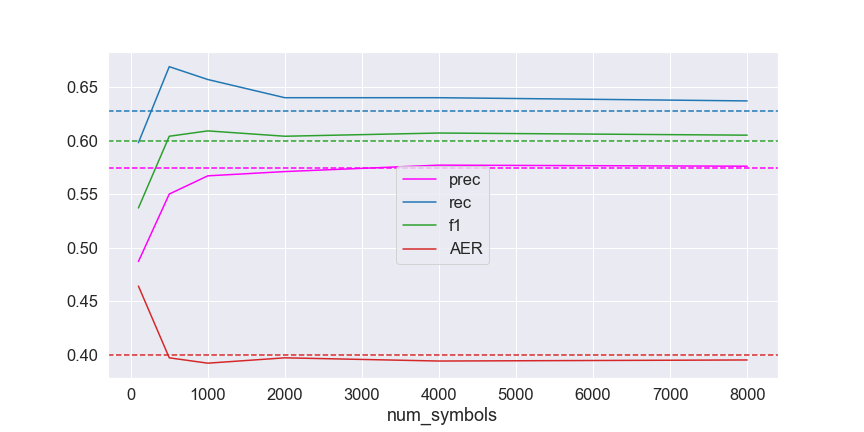
\includegraphics[width=14cm]{figures/eng_deu_fastalign.png}
    \caption{Scores of BPE over baseline}
\end{figure}

\section{Replication of BPE dropout}\label{sec:replbpedrop}

BPE dropout's difference with regards to normal BPE is the fact that some merges don't take place. Based on this randomness, each time this system is carried out, new BPE merges are created. For example, if the most merge in English \emph{(\_t, h)} wasn't merged, the resulting file of BPE merges would be vastly different than if the 10th most frequent merge didn't take place. In order to maintain some balance, the dropout algorithm is run a number of times, in this case 10 times, and then the alignments aggregated, which will be explained below. The algorithm to create the merge list remains unchanged, the first slight change occurs when applying the BPE algorithm to the corpus.

In the apply BPE algorithm, a random variable is created for every merge: if it falls below a threshold, the merge in question is discarded. And this function is repeated a number of times, creating a number of BPE files.

When extracting alignments, since now there are 10 BPE files instead of a single one, the whole algorithm is run 10 times, and alignments for all numbers of merges x all dropout repetitions are saved.

At this point, there are a number of alignments for each dropout case. Which alignment file to pick, or which ones, is the next step to be resolved. Three methods are selected:

\begin{itemize}
	\item Create the union of all alignments.
	\item Create the intersection of all alignments.
	\item Create a threshold parameter, for example 0.5. If an alignment is present in 50\% of the alignment files, it's added to the aggregated file.
\end{itemize}

To illustrate this with a example:

\begin{itemize}
	\item File 1: 0-0 0-1 1-1 1-2 2-3
	\item File 2: 0-0 0-1 1-2
	\item File 3: 0-0 1-1 1-3
	\item Union file: 0-0 0-1 1-1 1-2 1-3 2-3
	\item Intersection file: 0-0
	\item Aggregated file: 0-0 0-1 1-1 1-2
\end{itemize}

As it's visible in the example, the union case takes all alignments into account. By brute force, possibly most of the correct alignments will be present in the alignment (high recall), but the majority of the alignments in the union file will be incorrect (low precision). By contrast, the intersection file is the opposite. The file is much shorter since only the alignments present in \textbf{all} files are considered, these alignments will mostly be correct. But also many of the correct alignments will be missed. The aggregated file with the threshold aims to alleviate this problem by creating a sort of middle point between union and intersection.

\begin{python}

\end{python}

\begin{quote}
	a\\
\end{quote}

\begin{enumerate}
	\item 
\end{enumerate}